\subsection{Закон сохранения энергии и типы орбит}
Для движения тела в гравитационном массы $m$ в поле массы $M$ со 
скорость $v$ на расстоянии $r$ от гравитационного центра
справедливо следующее соотношение: \begin{equation}
\frac{m v^2}{2}-\frac{GM m }{r}=E_0,
\end{equation}
где $E_0$ --- константа, равна сумме кинетической и 
потенциальной энергии тела.

Если $E_0>0$, то траектория тела --- {\itshape гипербола}, 
ветви которой асимптотически приближаются к двум прямым.

Если $E_0=0$, то траектория тела --- {\itshape параболу}. При 
параболической и гиперболический траекториях движение не 
ограничено.

Если $E_0<0$, то траектория тела --- {\itshape эллипс}. При 
эллиптической траектории движение ограничено.

Параболическая скорость --- минимальная скорость, при которой 
тело покидает центральную массу $M$. Она также называется
{\itshape вторая космическая скорость}. Выражение для нее 
имеет следующий вид:\begin{equation}
v_{2}=\sqrt{\frac{2GM}{r}}
\end{equation}

На рис. 1 представлены примеры возможных траекторий тела 
относительно центрального (точка C).

При $v_0 > v_{2}$ (параболическая скорость) --- тело движется 
по гиперболе, при $v_0 = v_{2}$ --- тело движется по параболе, 
а при $v_0 < v_{2}$ --- по эллипсу.
\begin{figure}[h!]
\centering
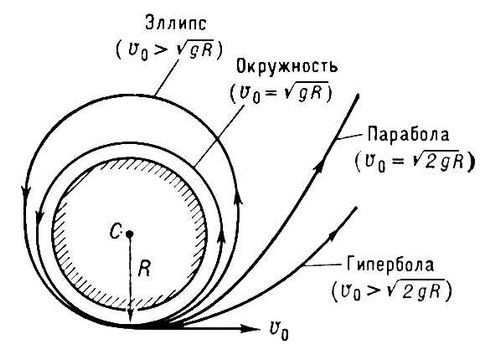
\includegraphics[width = 0.5\textwidth]{Space-speed}
\caption{Возможные траектории тела}
\end{figure}